\documentclass[a4paper, 11pt, oneside, german]{article}
\usepackage{gfsbaskerville}
% Load encoding definitions (after font package)
\usepackage[LGR,T1]{fontenc}
\usepackage{textalpha}
\usepackage{tabularx}
\usepackage{float}

\usepackage{listings}
\lstset{basicstyle=\ttfamily}
\usepackage{longtable}

\usepackage[dvipsnames]{xcolor}
\usepackage{eso-pic,graphicx}
\usepackage[top=80mm, bottom=70mm, outer=28mm, inner=28mm]{geometry}
\setlength{\columnsep}{90pt}

\definecolor{customColor}{RGB}{219, 219, 220}

\usepackage{sectsty}
\usepackage[titles]{tocloft}

\usepackage{setspace}
\onehalfspacing

% Babel package:
\usepackage{babel}
\usepackage{yfonts}
\usepackage{booktabs}
\setlength{\emergencystretch}{15pt}
\usepackage{fancyhdr}
\usepackage{microtype}
\usepackage{sectsty}

\sectionfont{\Huge}
\subsectionfont{\LARGE}
\subsubsectionfont{\Large}
\paragraphfont{\normalsize}

% change color of text, example replace all \color{Goldenrod} with \color{lightgray}

\makeatletter % change only the display of \thepage, but not \thepage itself:
\patchcmd{\ps@plain}{\thepage}{\bfseries\large\color{customColor}{\thepage}}{}{}
\makeatother

\color{customColor}

\begin{document}
\swabfamily
\renewcommand\thefootnote{{\arabic{footnote}}}
\let\oldfootnote\footnote
    \renewcommand{\footnote}[1]{\oldfootnote{\large#1}}
\AddToShipoutPictureBG{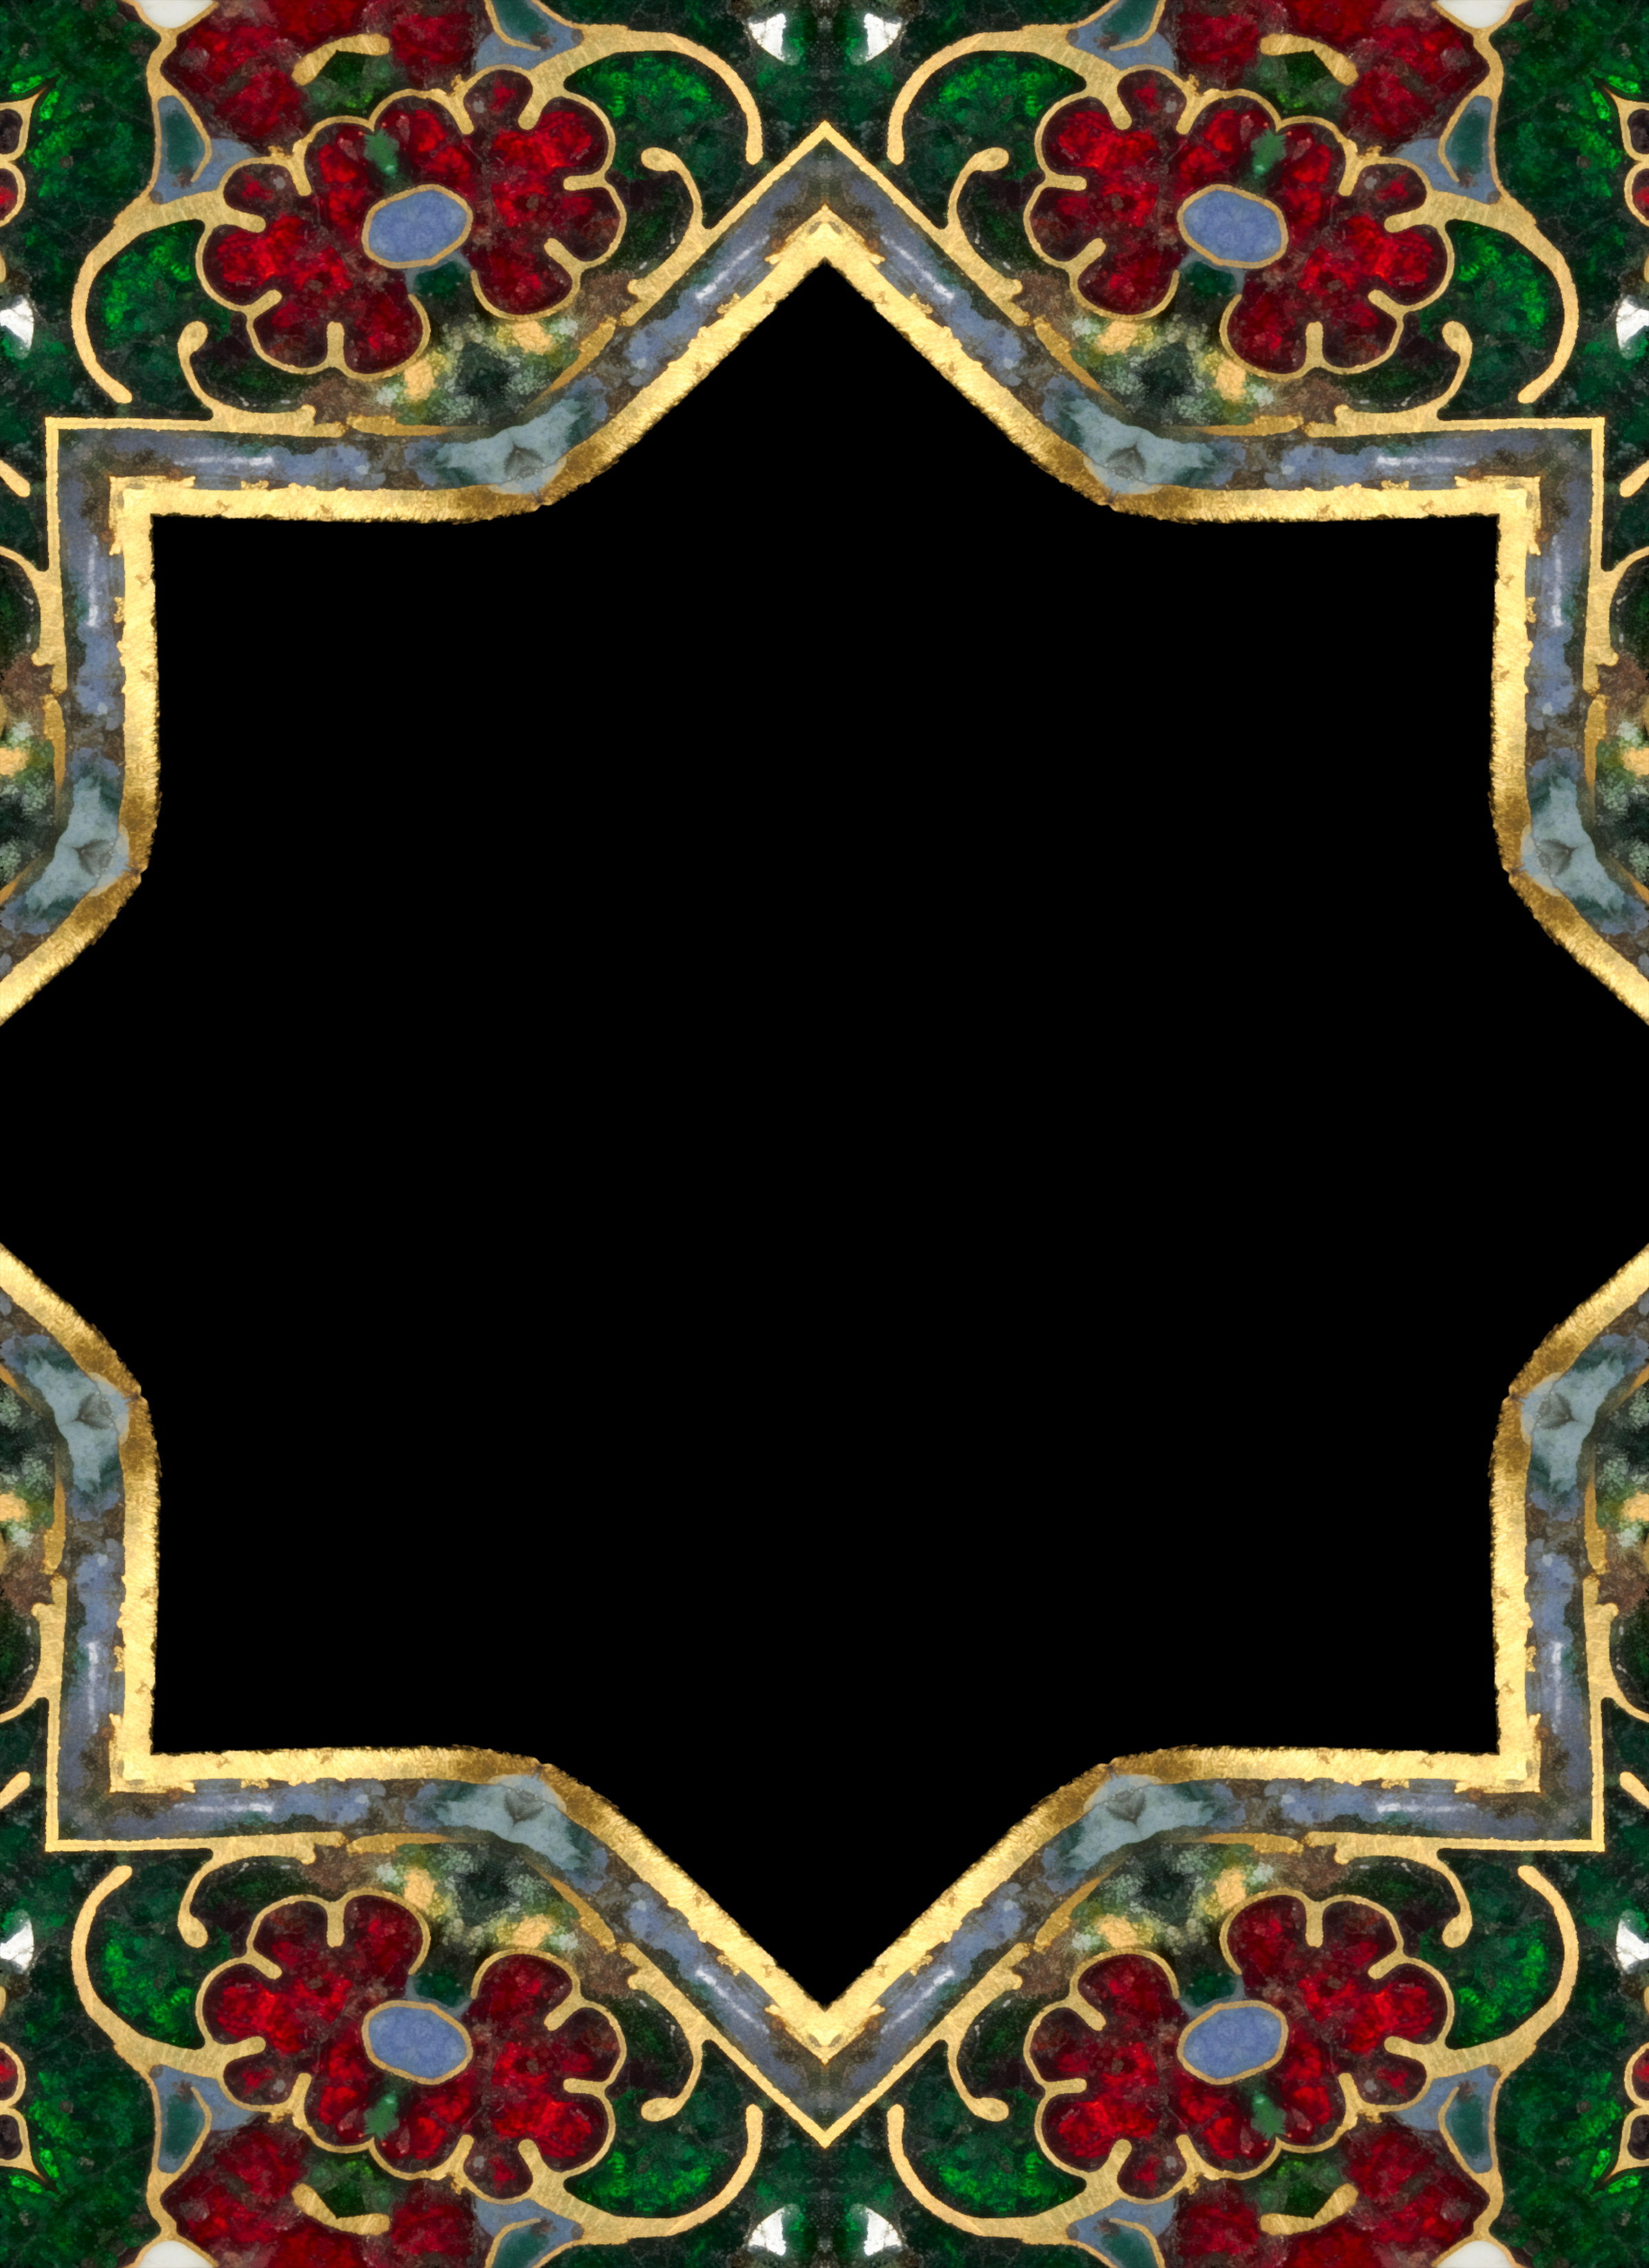
\includegraphics[width=\paperwidth,height=\paperheight]{paneljewel3.jpeg}}
\begin{titlepage} % Suppresses headers and footers on the title page
	\centering % Centre everything on the title page
	%\scshape % Use small caps for all text on the title page

	%------------------------------------------------
	%	Title
	%------------------------------------------------
	
	\rule{\textwidth}{1.6pt}\vspace*{-\baselineskip}\vspace*{2pt} % Thick horizontal rule
	\rule{\textwidth}{0.4pt} % Thin horizontal rule
	
	\vspace{1\baselineskip} % Whitespace above the title
	
	{\scshape\Huge "Uber die Meteoriten und ihre Beziehungen zur Erde.\\[1.25pt]}
	
	\vspace{1\baselineskip} % Whitespace above the title

	\rule{\textwidth}{0.4pt}\vspace*{-\baselineskip}\vspace{3.2pt} % Thin horizontal rule
	\rule{\textwidth}{1.6pt} % Thick horizontal rule
	
	\vspace{1\baselineskip} % Whitespace after the title block
	
	%------------------------------------------------
	%	Subtitle
	%------------------------------------------------
	
		
    {\scshape\large Von Prof. Karl Rammelsberg.} % Subtitle or further description
    
	%------------------------------------------------
	%	Editor(s)
	%------------------------------------------------
    \vspace*{\fill}

	\vspace{1\baselineskip}

	{\small\scshape Berlin 1872.}
	
	{\small\scshape{C. G. L"uderitz'sche Verlagsbuchhandlung.}}
	
	\vspace{0.5\baselineskip} % Whitespace after the title block

    \scshape Internet Archive Online Edition  % Publication year
	
	{\scshape\small Namensnennung Nicht-kommerziell Weitergabe unter gleichen Bedingungen 4.0 International} % Publisher
\end{titlepage}
\setlength{\parskip}{1mm plus1mm minus1mm}
\clearpage
\pagestyle{fancy}
\fancyhf{}
\cfoot{\swabfamily{\thepage}}
\Large
\paragraph{}
Nach physikalischen und chemischen Gesetzen kann sich die Gesamtmenge der materiellen Stoffe unserer Erde weder vermehren noch vermindern; es verschwindet nichts, es kommt nichts hinzu; jede Wandelung im Gebiet des Materiellen ist entweder eine physikalische "Anderung des molekularen Zustandes oder eine chemische Umsetzung der Bestandteile der K"orper.

Und dennoch hat die feste Masse des Erdk"orpers seit langer Zeit eine Vermehrung erfahren, und erf"ahrt eine solche noch immer. Ist die Gr"o"se dieses Zuwachses auch an sich verschwindend klein gegen die Gesamtmasse der Erde, so muss sie doch einen, f"ur jetzt allerdings noch nicht bemerkbaren Einfluss auf die Beziehungen unseres Planeten zu den "ubrigen K"orpern des Sonnensystems aus"uben. Wir meinen die Meteoriten, jene Stein- und Eisenmassen, welche von au"sen her durch die Atmosph"are hindurch auf die Oberfl"ache der Erde niederfallen.

Die Atmosph"are oder Lufth"ulle, welche die feste Masse und die fl"ussige Wasserbedeckung der Erdkugel umgibt, besteht bekanntlich aus einem "uberall gleichartigen Gemenge von Stickgas und Sauerstoffgas und enth"alt eine ver"anderliche Menge Wasserdampf. Wenn sich ein Teil dieses Dampfs in Folge von Abk"uhlung in feine dampfgef"ullte Bl"aschen fl"ussigen Wassers verwandelt, so wird er als Nebel oder Wolken sichtbar, kehrt aber durch den Einfluss der W"arme in den fr"uheren unsichtbaren Zustand zur"uck.

Was aus der Luft auf die Erde herabf"allt, ist im Wesentlichen niemals etwas Anderes als Wasser, entweder fl"ussiges (Regen) oder festes (Schnee, Hagel), und beide sind das Produkt einer raschen und massenhaften Abk"uhlung des in der Luft enthaltenen Wasserdampfs.

Unter besonderen Umst"anden werden auch andere K"orper von der Erde in die Luft gef"uhrt und k"onnen dann aus ihr wieder zur Erdoberfl"ache zur"uckkehren. Wenn ein Vulkan aus seinem Krater gl"uhende Lavabrocken in die H"ohe schleudert, so fallen die gr"o"seren St"ucke in der N"ahe herab und bedecken die Umgebung, die kleineren und feineren Teile aber werden von den Luftstr"omungen weiter fortgef"uhrt, und die kleinsten staubartigen Teilchen, welche man sehr unpassend "`vulkanische Asche"' nennt, verbreiten sich auf unglaublich weite Entfernungen. Heftige St"urme wirbeln den feinen Staub von der Oberfl"ache und tragen ihn "uber gro"se Landstrecken. Alle K"orper dieser Art, welche an Orten, denen sie ihren Ursprung nicht verdanken, zur Erde fallen, sind immer sehr leicht und unzweifelhaft als irdische (tellurische) Stoffe zu erkennen. "Uber ihre Herkunft herrscht kein Zweifel.

Ist es aber auch denkbar, dass K"orper, welche der Erde nicht angeh"oren (kosmische Substanzen), von au"sen her, aus dem Weltraum, in die Atmosph"are und durch diese hindurch auf die Erde gelangen k"onnen? Oder in der Sprache des Volkes ausgedr"uckt: K"onnen Steine vom Himmel fallen?

Die Chinesen, Inder, Griechen und R"omer sind in dieser Hinsicht einstimmig. Chinesische Schriftsteller verzeichnen 16 Meteorsteinf"alle von der Mitte des 7. Jahrhunderts v. Ch. bis 333 n. Ch. Livius spricht in seinem Werke mehrfach von Steinregen in Italien, und wir m"ussen bekennen: seit dem h"ochsten Altertum, durch die glanzvollsten Kulturperioden der griechischen und r"omischen Welt, durch das Mittelalter gehen bis in die neuere Zeit zahlreiche Berichte von Feuermeteoren, welche unter heftigem Get"ose Steine zur Erde geschleudert haben.

W"ahrend aber f"ur das Volk das Fallen von Steinen aus der Luft eine Tatsache war und blieb, bildete sich im 17. und 18. Jahrhundert, als die Naturwissenschaften sich zu entwickeln begannen, bei den Gebildeten und den Gelehrten die Meinung, es sei eine Torheit an solche Dinge zu glauben; T"auschung und Aberglaube l"agen allen derartigen Berichten zum Grunde. Erst gegen das Ende des 18., des Jahrhunderts der Aufkl"arung, und im Anfange des jetzigen bewirkte ein Zusammentreffen g"unstiger Umst"ande, dass die Urteile der Gelehrten in das Gegenteil umschlugen, und heute ist die wissenschaftliche Forschung vollkommen einig mit der geschichtlichen "Uberlieferung und dem nie ersch"utterten Volksglauben: es fallen Steine herab, es regnet Steine.

Jeder kennt die Erscheinung der Sternschnuppen, aber nicht Jeder hat eine Feuerkugel gesehen. Die Sternschnuppen find in neuerer Zeit von Astronomen und Physikern sorgf"altig beobachtet worden; man hat nicht allein eine periodische Wiederkehr ihrer Schw"arme zu gewissen Zeiten wahrgenommen, sondern auch festgestellt, dass die Bewegung dieser leuchtenden Meteore von bestimmten Punkten au"serhalb der Atmosph"are ausgeht, und man ist jetzt allgemein der Ansicht, dass Sternschnuppen und Feuerkugeln kleine mit planetarischer Geschwindigkeit sich bewegende Massen sind, welche im Weltraum nach den Gesetzen der allgemeinen Anziehung kreisen und dabei teilweise in die N"ahe des Erdk"orpers gelangen. Werden sie von diesem angezogen, so m"ussen sie beim Durcheilen der Atmosph"are in Folge des Widerstandes der Luft sich bis zum Gl"uhen erhitzen und schlie"slich als Meteoriten niederfallen.

So h"atten wir denn Gelegenheit, K"orper in die Hand zu nehmen, welche, unserer Erde fremd, dem Weltraum entstammen; wir k"onnen ihre physikalischen und chemischen Eigenschaften pr"ufen, und wenn der blo"s beobachtende und rechnende Astronom alle wissenschaftlichen Hilfsmittel benutzt, um "uber die Stellung, die Gr"o"se und die Bewegung der Weltk"orper Aufschluss zu geben, wenn in neuester Zeit aus Spektralbeobachtungen sogar Schl"usse auf die materielle Beschaffenheit jener K"orper gezogen worden find, so bieten uns dagegen die Meteoriten die unerwartete Gelegenheit, die Natur kosmischer Substanzen durch Versuche zu ermitteln, und diese Erfahrungen sind es vorzugsweise, welche wir hier in ihren allgemeinen Resultaten vorf"uhren wollen.

Das Niederfallen von Meteoriten ist ohne alle Frage weit h"aufiger, als man nach den vorhandenen Beobachtungen schlie"sen darf. An keine Zeit und an keinen Ort der Erde gebunden, kann die Erscheinung sehr wohl statthaben, ohne ihren Beobachter zu finden. Selbst in bewohnten Gegenden ist dies m"oglich, um wie viel mehr aber in Urw"aldern, W"usten und Steppen, auf dem weiten Ocean oder auf dem Eise der Polarl"ander. Auch darf es nicht befremden, dass Meteoritenf"alle fast nur von Leuten aus dem Volke beobachtet wurden, dass Gebildete oder Gelehrte kaum jemals Augenzeugen der Erscheinung gewesen sind. Nur so konnte es geschehen, dass gerade in einem Zeitalter, welches sich der Aufkl"arung r"uhmte, alle Aussagen und Berichte "uber Meteoritenf"alle von den Fachgelehrten f"ur Fabeln und T"auschungen erkl"art wurden.

In der Tat sind die Erscheinungen beim Niederfallen von Meteoriten so eigent"umlicher Art, dass es f"ur unseren Zweck passend erscheint, ihrer zu gedenken, bevor wir von der materiellen Beschaffenheit dieser Fremdlinge auf der Erde reden. Wir w"ahlen einige hervorragende, genau konstatierte F"alle und beginnen mit dem Steinfall von Aigle, weil der Bericht, welchen der ber"uhmte Physiker Biot "uber ihn an die Pariser Akademie erstattete, diese gelehrte K"orperschaft endlich zwang, die Tatsache des Steinregens anzuerkennen.

Am 26. April 1803, Mittags zwischen 1 und 2 Uhr, sah man in Frankreich zu Alençon, Falaise, Caen und anderen Orten eine gro"se Feuerkugel, welche sich am heiteren Himmel von S"udost nach Nordwest bewegte. Einige Augenblicke nachher wurde bei l'Aigle im Departement de l'Orne eine kleine dunkle Wolke am Himmel gesehen, aus welcher 5 bis 6 Minuten lang eine Detonation, gleich dem Schall von grobem Gesch"utz, von Kleingewehrfeuer und von Trommelwirbel erfolgte, wobei einzelne Teile der Wolke sich von ihrem K"orper best"andig losrissen. W"ahrend dieser Explosionen erfolgte ein f"ormlicher Steinhagel; auf einer fast 2 Meilen langen Strecke fielen mit entsetzlichem Geprassel 2-3000 Steine nieder, deren gr"o"ster Kilogramm (18 Pfund) wog.

Durch Leblond, einen in l'Aigle wohnenden Korrespondenten der Pariser Akademie, ward die Aufmerksamkeit der gelehrten Welt auf das merkw"urdige Ereignis gelenkt; die Akademie sandte Biot, eins ihrer j"ungsten Mitglieder, nach dem Orte des Falles, und Biot untersuchte die Lokalit"at, sammelte die Aussagen der Zeugen --- fast s"amtlicher Bewohner von 20 D"orfern ---, brachte eine Anzahl der gefallenen Steine nach Paris und war vollkommen "uberzeugt, der Steinregen von l'Aigle sei das Resultat des sukzessiv erfolgten Zerplatzens des Meteors gewesen.

Am 14. Juli 1847, Morgens $3\frac{3}{4}$ Uhr, wurden die Bewohner der Stadt und Umgegend von Braunau in B"ohmen durch zwei einander folgende heftige Explosionen gleich Kanonensch"ussen aus dem Schlaf geschreckt. Am ganzen S"udrande des schlesisch-b"ohmischen Gebirges bis in die Grafschaft Glatz h"orte man zu dieser Zeit ein heftiges Sausen und Brausen in der Luft. Bei fast wolkenlosem Himmel gewahrte man "uber dem nord"ostlich von Braunau gelegenen Hauptmannsdorf eine kleine schwarze Wolke, welche pl"otzlich leuchtend wurde, zuckende Blitze nach allen Seiten und zwei Feuerstreifen nach abw"arts sandte, worauf die erw"ahnte Detonation erfolgte. Der Berichterstatter, der Oberf"orster Pollack, schloss auf einen Meteorsteinfall, die Mehrzahl der "ubrigen Beobachter jedoch dachte nur an eine Gewitterwolke und das Einschlagen des Blitzes.

In der Tat hie"s es, der Blitz habe 100 Schritt vom Dorfe in den Acker geschlagen; als man die Stelle untersuchte, lag in einem 3 Fu"s tiefen Loche eine gl"uhende Masse, "uber deren Herabst"urzen ein Augenzeuge, Joseph Tepper, einen Bericht zu Protokoll gab. Sechs Stunden nach dem Fall war diese Masse noch so hei"s, dass man sie nicht ber"uhren konnte. Sie wog 21,1 Kilogramm (46 Pfund 6 Loth) und wird im Wiener Mineralienkabinett aufbewahrt.

Gleichzeitig traf die Meldung ein, der Blitz habe ein Haus, eine Viertelstunde von Braunau, getroffen. Das Dach, das Holzwerk und der Estrich waren durchschlagen, und dies hatte eine 15,25 Kilo ($30\frac{1}{2}$ Pfund) schwere Masse getan, welche man auffand und die jener ersten vollkommen glich. Sie ist sp"ater in den Besitz des Klosters Braunau gelangt. Fragmente beider Massen aber finden sich in verschiedenen gr"o"seren Mineraliensammlungen.

Als ein Fall, welcher der neuesten Zeit angeh"ort, mag der Steinregen von Pultusk in Polen dienen, welcher sich am 30. Januar 1868 ereignete.

An diesem Tage um 7 Uhr Abends erschien bei fast heiterem Himmel eine gl"anzende Feuerkugel am Warschauer Horizont; sie wurde zuerst in S"udost nahe dem Kopf der Andromeda sichtbar, und hatte das Ansehen eines Sterns erster Gr"o"se, vergr"o"serte sich aber zusehends der Art, dass ihr Durchmesser beim Passieren des Warschauer Meridians 15 bis 20 Minuten betrug. Nachdem das Meteor durch Kassiopeia, Kepheus, den Drachen und bis zum Stern $\eta$ des gro"sen B"aren gegangen war, lie"s es einen Lichtschweif von 9 Grad L"ange und 2 Grad Breite hinter sich. Zugleich verwandelte sich das anfangs stern"ahnliche Licht beim Gr"o"serwerden der Kugel in Blaugr"un und dann in Dunkelroth, und die Intensit"at dieses Lichts war so gro"s, dass die Menschen auf die Stra"se eilten und den Widerschein einer Feuersbrunst zu sehen glaubten.

Dieses Feuermeteor ist gleichzeitig in Danzig, Posen, Krakau, Prag, Wien, Grodno und Dorpat beobachtet worden, und aus einigen dieser Beobachtungen hat man berechnet, dass es sich mit einer Geschwindigkeit von 6,6 Meilen in der Sekunde bewegt habe.

Drei Tage sp"ater erfuhr man in Warschau, dass 77 Kilometer (11 Meilen) in Nordosten entfernt, bei Pultusk eine Anzahl von Meteorsteinen gefallen sei, und es wurden Prof. Babczynski und der Adjunkt der Sternwarte, Deicke, an Ort und Stelle gesandt, um die n"aheren Umst"ande zu erforschen und die Meteoriten zu sammeln. Danach hatte man die Feuerkugel in der Gegend von Pultusk gleichfalls an jenem Tage um 7 Uhr Abends in Form eines Sterns beobachtet, der sich mit Schnelligkeit von S"udost nach Nordwest bewegte und einen funkenspr"uhenden Streifen nach sich zog. Auch hier nahm die scheinbare Gr"o"se und die Lichtst"arke des Meteors ungemein rasch zu, und zwar letztere in dem Grade, dass sie das Auge blendete. Pl"otzlich verschwand die Kugel, es fielen leuchtende Punkte herab, und an ihrer Stelle erschien ein lichtes zackiges Gew"olk, von welchem einzelne Donnerschl"age und ein anhaltendes Rollen w"ahrend einer halben Minute ausgingen. Zu gleicher Zeit aber vernahm man in den nahen D"orfern am Ufer des Narew das Prasseln und Sausen herabfallender Steine und ihr Aufschlagen auf das Eis und das "uber demselben stehende Wasser.

Das Meteor war also auch hier unter gewaltiger Explosion in zahllose Bruchst"ucke zersprungen, welche eine Bodenfl"ache von 16 Quadratkilometern bedeckten. Etwa 400 St"uck wurden gesammelt, unter ihnen ein Stein von 7 Kilogramm, drei andere von je 4 Kilogramm Gewicht; allein ein gro"ser Teil war auf die vom Wasser bedeckten Wiesen und in den Fluss gefallen. Man sch"atzt ihre Gesamtmasse auf 5-600 Kilogramm.

Die hier gegebene Schilderung der Meteoritenf"alle von l'Aigle, von Brannau und von Pultusk passt auf die meisten "ubrigen; allein man darf nicht vergessen, dass die "alteren Berichte den Charakter vieler historischen Nachrichten an sich tragen, dass "Ubertreibungen und Entstellungen und die Produkte einer erregten, an Zeichen und Wunder glaubenden Phantasie reichliche Nahrung in solchen Naturerscheinungen gefunden haben.

Zun"achst ist die Frage: Sind alle Meteoriten K"orper gleicher Art? Die Antwort lautet: Nein. Bei l'Aigle und Pultusk fielen Meteorsteine, bei Braunau fiel Meteoreisen. Es gibt also zwei Klassen von Meteoriten: die einen haben die Beschaffenheit der gew"ohnlichen Mineralien (Steine), die anderen find von der Natur des metallischen Eisens.

Das Herabfallen dieser Art, des Meteoreisens, ist selten beobachtet worden. Au"ser dem Fall von Braunau kennen wir einen solchen zu Hraschina bei Agram in Kroatien am 16. Mai 1751 und einen im Jahre 1835 im Staat Tennessee in Nordamerika. Dass aber auch zu anderen Zeiten Meteoreisen niedergefallen sei, daf"ur sprechen die teilweise kolossalen Eisenmassen, welche man in einzelnen Gegenden der Erde teils auf der Oberfl"ache, teils in geringer Tiefe gefunden hat. Dass auch sie meteorischen Ursprungs find, beweist die "Ubereinstimmung ihrer chemischen Natur mit jenen Massen von Braunau und Agram und der Umstand, dass sie an Orten vorkommen, wo sie unm"oglich von jeher sich befunden haben k"onnen. Solche gr"o"sere Eisenmassen erhalten sich unver"andert im Laufe der Jahrtausende, nur ihre Oberfl"ache "uberzieht sich mit einer Rostschicht. Ganz anders verh"alt es sich mit den eigentlichen Meteorsteinen, welche, wenn sie unbeachtet liegen bleiben, allm"ahlig verwittern, zerfallen und ganz unkenntlich werden. Aus diesem Grunde enthalten unsere Sammlungen nur solche Meteorsteine, deren Fallzeit man kennt, dagegen aber sehr viele Meteoreisen, von welchen nur der Fundort bekannt ist.

Wie Jeder wei"s, ist das Eisen ein auf oder vielmehr in der Erde "au"serst h"aufiges Metall; es wird daher die Frage laut werden: Warum sind jene gro"sen Eisenmassen nicht Angeh"orige der Erde?

Metallisches Eisen (Stab- oder Schmiedeeisen) gewinnen wir durch Schmelzprozesse aus Eisenerzen, d. h. aus chemischen Verbindungen des Eisens mit Sauerstoff. Nur in Verbindung mit Sauerstoff oder mit Schwefel finden wir das Eisen in der Erde, d. h. in denjenigen Teilen der gro"sen Erdmasse, auf welche unsere Kenntnis und unsere bergm"annischen Arbeiten sich beschr"anken. Niemals haben sich auf Eisenerzlagerst"atten oder "uberhaupt im festen Gestein Andeutungen von metallischem Eisen gefunden, aus welchem jene Bl"ocke bestehen, welche auf dem Kamm von Gebirgen, oder in T"alern, in W"usten fern von allen Eisenerzen freiliegend gefunden werden.

Weit "uberzeugender f"ur den meteorischen Ursprung solcher Eisenmassen ist ihr best"andiger Gehalt an einem anderen Metall dem Nickel, dessen Menge bei sehr vielen 10 Prozent ausmacht. Dieser Nickelgehalt charakterisiert die Eisen von Agram und Braunau, deren Fall erwiesen ist, gleichwie alle jene, welche in Bezug auf ihre Fallzeit unbekannt sind. L"ost man solches Eisen in einer S"aure auf, so bleibt fast immer ein kleiner Rest zur"uck, und in diesem weist die chemische Untersuchung gleichfalls Eisen und viel Nickel, aber zugleich Phosphor nach. Derartige Erscheinungen zeigen weder die Eisenerze noch das aus ihnen dargestellte metallische Eisen.

Unter der Regierung der Kaiserin Katharina von Russland bereiste der ausgezeichnete Naturforscher Peter Simon Pallas, ein Berliner, die weiten Landstrecken Sibiriens, und fand im J. 1771 auf einem H"ohenzuge zwischen dem Ubei und Sisim. Nebenfl"ussen des Jenisei, eine gro"se Eisenmasse, welche schon 1749 von Medwedew bemerkt worden war. Er lie"s sie nach Krasnojarsk bringen, von wo sie sp"ater nach Petersburg kam. Diese Masse, welche unter dem Namen der Pallasmasse bekannt ist, soll urspr"unglich ein Gewicht von 688 Kilogr. gehabt haben, ist aber jetzt nach Abgabe zahlreicher St"ucke an die verschiedensten Sammlungen um Vieles leichter.

Diese Pallasmasse ist in doppelter Beziehung von Interesse. Sie bildet n"amlich so zu sagen ein Mittelglied zwischen Meteoreisen und Meteorsteinen. Es ist eine von lauter H"ohlungen durchsetztem Masse von Meteoreisen, und diese H"ohlungen sind ausgef"ullt mit einem gr"ungelben, kristallisierten Mineral, dem Olivin, welches in den eigentlichen Meteorsteinen fast nie fehlt. Sp"ater haben sich auch in anderen Gegenden ganz "ahnliche Durchwachsungen von Meteoreisen und Olivin gefunden.

Die Pallasmasse gab einem deutschen Physiker, dem Prof. Chladni in Wittenberg, zuerst den Gedanken ein, sie sei meteorischen Ursprungs, es gebe "uberhaupt Meteormassen, ihr Herabfallen sei keine Fabel. Von seinen gelehrten Zeitgenossen verspottet, hat Chladni, wie wir weiterhin sehen werden, dennoch sehr bald die Zustimmung der wissenschaftlichen Welt erlangt.

Seit dem Ende des 14. Jahrhunderts bewahrte man auf dem Rathause zu Elbogen in B"ohmen eine 95,5 Kilogr. (191 Pfund) schwere Masse auf, welche "`der verw"unschte Burggraf"' hie"s. In neuerer Zeit als Meteoreisen erkannt, ist sie der Wiener Sammlung einverleibt worden. Im Dorfe La Caille, Dépt. du Var, lag ein Block von 591 Kil. Schwere seit undenklicher Zeit vor der Kirchenpforte und diente als Sitz, bis er 1848 als ein sch"ones Exemplar Meteoreisen in das Pariser Musée d'histoire naturelle wanderte. Bei einem Wegebau in der Gegend von Bitburg, n"ordlich von Trier, fand sich 1802 eine Eisenmasse von 1650 bis 1700 Kil. (32-34 Ztr.); man schaffte sie nach einer Eisenh"utte (dem Pluwiger Hammer), um sie im Feuer zu verarbeiten, und als dies nicht gl"uckte, wurde sie bei Seite geworfen, so dass jetzt, nachdem ihre Natur als Meteoreisen erkannt ist, nur noch geringe Reste der urspr"unglichen, nicht durch das versuchte Einschmelzen ver"anderten Masse vorhanden find, und diese lassen auf eine gewisse "Ahnlichkeit mit der Pallasmasse schlie"sen. Ein ganz "ahnliches Schicksal hat ein 246 Kilogr. schwerer Eisenblock gehabt, welchen Bauern in 2 Fu"s Tiefe beim Dorfe Netschaewo, nahe bei Tula in Russland, fanden und an eine Eisenh"utte verkauften. Erst 1857 wurde der nicht verarbeitete Teil von Dr. Auerbach aus Moskau als Meteoreisen erkannt und f"ur die Wissenschaft gerettet.

Von Meteoreisenfunden aus gr"o"serer N"ahe wollen wir nur eine im Wiesengrund bei Seel"asgen (Kreis Schwiebus) ausgegrabene, lange unbeachtet gebliebene und 1847 erkannte Masse, sowie ein 20 Kilogr. schweres St"uck erw"ahnen, welches man beim Bau der Ostbahn 1850 in der N"ahe von Schwetz in dem Sand und Lehm des hohen Weichselufers fand.

Diese Meteoreisen find ihrer Masse nach unbedeutend, im Vergleich zu gewissen amerikanischen. Westw"arts der Stadt Mexico, im Thal von Toluca, liegen viele und gro"se Eisenmassen, welche schon vor der Ankunft der Spanier im Lande zu Ger"atschaften verarbeitet wurden. A. v. Humboldt hat Proben davon nach Europa gebracht. Im Innern der argentinischen Staaten, in der "oden Gegend von S. Iago del Estero, liegen Eisenmassen bis zu 15,000 Kilogr. Gewicht.

In der letzten Zeit hat ein Vorkommen gro"ser Eisenmassen in Gr"onland vielfach von sich reden gemacht. Es wurden n"amlich im J. 1870 durch eine schwedische Expedition auf der Insel Disko dicht am Meeresstrande nicht nur drei gr"o"sere Bl"ocke gefunden, deren Gewicht auf 25,000, 10,000 und 4500 Kilogr. gesch"atzt wurde, sondern noch eine Anzahl kleinerer St"ucke in n"achster N"ahe. Im Jahre 1871 hat man die Massen nach Europa gebracht und den gr"o"sten Teil in dem Stockholmer Museum aufgestellt.

Wie schon angef"uhrt, ist jedes Meteoreisen im Wesentlichen eine Legierung von Eisen und Nickel, welche die allgemeinen Eigenschaften des geschmeidigen Eisens, des Stab- oder Schmiedeeisens zeigt. Doch ist das Meteoreisen durch sein inneres Gef"uge, seine Struktur, so gut charakterisiert, dass sich seine Natur auch hierdurch zu erkennen gibt. Schneidet man ein St"uck durch, poliert die ebene Schnittfl"ache und taucht sie einige Minuten in eine verd"unnte S"aure, so gewahrt man auf ihr eigent"umliche, h"ochst zarte Linien und Figuren, welche nach ihrem Entdecker die Widmannst"atten'schen Figuren hei"sen. Sie beweisen, dass die ganze Masse aus d"unnen Lagen einzelner Krystalle besteht, und dass das Ganze auch in chemischer Beziehung nicht gleichartig ist, sondern dass einzelne Teile von der S"aure leichter aufgel"ost werden als andere. Selten ist es, dass das ganze St"uck des Meteoreisens gleichsam nur einen einzigen Kristall (freilich ohne "au"sere Fl"achen) bildet, wie dies z. B. bei dem Eisen von Braunau der Fall ist; dann sind auch jene Linien anderer Art. Jedoch auch in diesem Fall ist die Hauptmasse des Eisens mit einer nickelreicheren Legierung in mikroskopischen Krystallen durchsetzt, welche sich in S"auren schwerer aufl"osen und dabei sichtbar werden.

Den Gegensatz zum Meteoreisen bilden die eigentlichen Meteorsteine, welche, wie wir an den Beispielen von l'Aigle und Pultusk sahen, "ofter in gro"ser Zahl durch das Zerplatzen eines einzigen Meteors umhergestreut werden, obwohl in den meisten F"allen nur einige Steine, Bruchst"ucke eines gr"o"seren, herabst"urzen, oder selbst nur ein einzelner Stein zur Erde f"allt. Woraus bestehen nun diese Massen? Im Allgemeinen haben sie eine gewisse "Ahnlichkeit mit unseren kristallinischen Gebirgsarten, insofern sie in der Regel gleich diesen aus mehreren Mineralien bestehen. Und doch stimmen sie mit keinem der irdischen Gesteine "uberein. Auch sind sie nicht alle gleicher Art, und wir wollen versuchen, im Nachfolgenden einen Begriff von ihrer eigent"umlichen Beschaffenheit zu geben.

Die feste Masse unserer Erde, welche wir in Gebirgen oder am Meeresufer oder beim Eindringen in die Tiefe (in Bergwerken, bei der Anlage von Tunnels oder tiefen Einschnitten) vor uns sehen, wird von mannigfachen Gesteinen oder Gebirgsarten gebildet. Ein solches Gestein kann aus einem einzelnen Mineral bestehen, welches in Folge seiner gro"sen r"aumlichen Verbreitung den Charakter einer Gebirgsart angenommen hat. So bildet der k"ornige Kalk (der wei"se Marmor) in der Gegend von Carrara hohe Gebirge. Eine andere Art Kalkstein, von dichter Masse und in Lagen oder Schichten abgesondert, findet sich "ostlich von Berlin, bei R"udersdorf, und ist als Baumaterial von gro"ser Wichtigkeit. Andere Gebirgsarten bestehen aus mehreren Mineralien, welche oft schon das unge"ubte Auge leicht unterscheidet. Zu ihnen geh"ort der Granit. Ein St"uck Granit, gleichviel, ob wir es im Ilztal des Harzes, oder im Riesengebirge, oder unter den losen Bl"ocken der norddeutschen Ebene auflesen, l"asst immer drei verschiedene Mineralien in seiner Masse unterscheiden: den r"otlichen Feldspat, den grauen fettgl"anzenden Quarz und die d"unnen wei"sen, braunen oder schwarzen Bl"attchen des Glimmers. Der Kalkstein ist ein einfaches, der Granit ein gemengtes Gestein. Die Gemengteile sind einzelne Mineralien; durch sie unterscheiden sich die verschiedenen gemengten Gesteine, und die Kenntnis der letzteren beruht auf der Kenntnis der sie bildenden einzelnen Mineralien. Genau ebenso verh"alt es sich mit den Meteorsteinen.

Die bei Weitem gr"o"ste Zahl der zu verschiedenen Zeiten und an verschiedenen Orten gefallenen Steine geh"ort einer und derselben Art an. Oberfl"achlich betrachtet, erscheinen sie als eine hellere oder dunklere graue Masse, in welcher kleinere oder gr"o"sere K"ugelchen liegen, welche ihnen den gemeinsamen Namen "`Chondrite"' verschafft haben. Nimmt man aber die Lupe oder das Mikroskop zu H"ulfe, so sieht man, dass die Masse aus verschiedenen Mineralien besteht, und bei vielen lassen sich gelbliche oder gr"unliche K"ornchen neben wei"sen, grauen oder br"aunlichen unterscheiden. Zahlreiche mineralogische und chemische Untersuchungen haben gelehrt, dass dies zwei Mineralien sind, welche im Wesentlichen aus Kiesels"aure, Magnesia und Eisenoxydul, jedoch in abweichenden Verh"altnissen, bestehen; die gr"unlich-gelben K"orner sind Olivin, die anderen Bronzit, und beide kommen auch in irdischen Gesteinen h"aufig vor. Aber die Chondrite enthalten noch einen Gemengteil, welcher den bekannten Gesteinen der Erde fehlt, dies ist metallisches nickelhaltiges Eisen, d. h. Meteoreisen in feineren und gr"oberen Teilchen, und dieses Gemengteil gen"ugt, um sie als Meteoriten zu erkennen.

Sehr interessant ist der seltene Fall, dass Olivin und Bronzit in gr"o"seren kristallinischen Massen, welche zugleich das Eisen umschlie"sen, nebeneinander liegen, und sich leicht erkennen und getrennt untersuchen lassen. Solche "`Mesosiderite,"' wie man sie genannt hat, sind bei ihrem Fallen bisher nicht beobachtet, sondern ein gl"ucklicher Zufall hat zu ihrer Auffindung gef"uhrt, so bei Hainholz unweit Paderborn, wo ein ansehnlicher Block im Ackerlande gefunden wurde; in den "oden Gebirgen des n"ordlichen Chile, von wo sie durch Reisende bekannt geworden sind.

Gleichwie bei den Gebirgsarten der Erde die n"amlichen Gemengteile in der Gr"o"se der Teilchen und in den Mengenverh"altnissen vielfach variieren k"onnen, so auch bei den Meteoriten. Und so wie bei jenen h"aufig ein Gemengteil seiner Menge nach zur"ucktritt und endlich ganz fehlt, so dass nun eine andere Gebirgsart vorliegt, so kennen wir unter den Meteoriten auch blo"se Gemenge von Meteoreisen und Olivin, oder von Meteoreisen und Bronzit. Zu jenen geh"ort die schon erw"ahnte Pallasmasse, eine ganz "ahnliche von Brahin und eine von Atacama in S"udamerika; zu diesen mehrere Massen, welche man zu Breitenbach, Rittersgr"un und Steinbach im Erzgebirge gefunden hat, denn bei keinem dieser Meteoriten ist das Herabfallen nachgewiesen. Das Eisen bildet in ihnen eine Art Skelet, in dessen zahllosen H"ohlungen das eine oder andere Mineral in Krystallen steckt.

Am 30. November 1850 fiel bei Shalka in Bengalen ein Meteorstein, welcher nur aus Olivin und Bronzit besteht, dem also das Meteoreisen fehlt.

Am 3. Oktober 1815 beobachtete man bei Chassigny, s"ud"ostlich von Langres im Dépt. Haute-Loire, bei sonst heiterem Himmel aus einer grauen Wolke unter heftigem Get"ose das Fallen zweier Steine, und diese bestehen nur aus Olivin.

Die beiden am 26. Juli 1843 bei Manegaum in Ostindien gefallenen Steine und der am 17. Juni 1870 bei Ibbenb"uhren in Westphalen gefallene 2 Kilogr. schwere Stein bestehen lediglich aus Krystallk"ornern von Bronzit.

Aus ganz anderen Mineralien find gewisse Meteorsteine zusammengesetzt, welche die Klasse der "`Eukrite"' bilden.

Am 22. Mai 1808 ereignete sich bei Stannern unweit Iglau in M"ahren ein Steinregen, bei welchem unter heftigen Detonationen eine Feuerkugel mit Schweif in drei Intervallen zerplatzte, und eine Strecke Landes mit Hunderten von Steinen bedeckte. Die Wiener Sammlung enth"alt ihrer 61 und der gr"o"ste wiegt fast 14 Kilogramm. --- Bei Jonzac, nahe Barbézieux im Dépt. Charente inférieure, fielen am 13. Juni 1819 und bei Juvinas im Dpt. Ardèche am 15. Juni 1821 Meteorsteine derselben Art, am letzteren Orte ein gro"ser Stein von 110 Kilogramm neben einigen kleineren. Diese Meteorsteine find ein Gemenge von zwei zum Teil wohlkristallisierten Mineralien, einem braunen, Augit, und einem wei"sen, Anorthit, neben welchen kleine Krystalle von Magnetkies (Schwefeleisen) bemerkt werden. Der Augit besteht aus Kiesels"aure, Eisenoxydul, Magnesia und Kalk, das Anorthit aus Kiesels"aure, Tonerde und Kalk.

Hiermit ist jedoch die Mannigfaltigkeit der Meteoritenmischung nicht ersch"opft. Die Steine, welche am 13. Dezember 1813 bei Luotolax in Finnland niederfielen, bestehen aus Olivin, Augit und Anorthit, und die von M"assing in Bayern (13. Dezember 1803), von Białystok in Russland (17. Oktober 1827) und von Nobleborough im Staat Maine (7. August 1823) geh"oren zu derselben Art, welche man "`Howardite"' genannt hat.

Die schwarze Rinde, welche die Meteorsteine umgibt, muss als ein Produkt der Schmelzung ihrer Oberfl"ache angesehen werden.

Die Mineralien, aus welchen die Meteorsteine bestehen, find mit Ausnahme des metallischen nickelhaltigen Eisens lauter bekannte Mineralien, d. h. solche, welche in irdischen Gesteinen l"angst bekannt sind. Alle Elemente, welche in den Meteoriten bisher nachgewiesen find, sind bekannte. Dieser Umstand ist von gro"ser Bedeutung, denn er l"asst vermuten, dass die Anh"aufungen fester Materie im Sonnensystem aus denselben Elementen und denselben chemischen Verbindungen bestehen, und dient der Hypothese von Kant und Laplace zur St"utze, wonach die Sonne und die sie umkreisenden Weltk"orper aus der Verdichtung einer urspr"unglichen Dampfmasse entstanden sind.

Kehren wir von der Betrachtung der materiellen Natur der Meteoriten einen Augenblick zu den Erscheinungen zur"uck, welche ihrer Ankunft auf der Erde unmittelbar voraufgehen. Ein leuchtendes Meteor erscheint am Himmel; heftige Donnerschl"age ert"onen und werden meilenweit vernommen; prasselnd st"urzen einzelne oder viele Steine aus der Luft zur Erde und graben sich in die weiche Oberfl"ache tief ein; sie sind noch hei"s, wenn es gelingt sie in nicht allzulanger Zeit aufzufinden.

Haben ungew"ohnliche Erscheinungen in der Natur den Menschen von je her in Furcht gesetzt, so m"ussten Meteoritenf"alle diese Wirkung in besonders hohem Grade "au"sern. Bis in die neuere Zeit erstreckt sich der Einfluss solcher Erscheinungen gleichm"a"sig auf Alle, denn noch fehlte das Licht, mit welchem die Naturwissenschaften Aberglauben und Unwissenheit in den nat"urlichen Dingen bek"ampfen; die Lehrer der Schulen und der Universit"aten standen darin allen Anderen gleich, und die wenigen M"anner, welche sich mechanische, physikalische oder chemische Kenntnisse erworben hatten, liefen Gefahr, f"ur Zauberer gehalten und verfolgt zu werden. Diese Zeiten sind vor"uber, aber der Glaube an geheimnisvolle, dem Menschen feindliche M"achte, welche sich in Naturerscheinungen offenbaren, ist geblieben.

Als der oben erw"ahnte Steinfall von Juvinas sich ereignete, gerieten die Bauern auf dem Felde derma"sen in Angst, dass sie eine Rotte von Teufeln in der Luft zu h"oren vermeinten, in dem Glauben, ihre letzte Stunde sei gekommen, ihre Seele Gott empfahlen und den Tod erwarteten. Nur die Kinder verfolgten die Erscheinung, nur sie wussten nachher die Stelle anzugeben, wo der gro"se Stein in die Erde geschlagen war, aber acht Tage lang lie"s sich Niemand bewegen, ihn auszugraben, denn Alle glaubten, der Teufel halte sich in der N"ahe versteckt.

Die Mineralien der Meteorsteine sind solche, welche in den Laven unserer Vulkane und in kristallinischen Gesteinen der Erde vorkommen; wir schlie"sen hieraus, dass auch sie bei ihrer Bildung geschmolzen gewesen sein m"ussen. Als feste Massen aber haben sie sich im Weltenraume bewegt, bis sie in die N"ahe der Erde kamen. Gelangt ein fester K"orper in die Atmosph"are und bewegt sich in derselben gegen die Erde, so erleidet er durch die Luft einen Widerstand, welcher umso gr"o"ser ist, je schneller die Bewegung. Unter Annahme einer Fallgeschwindigkeit von 1 Kilometer (etwa $\frac{1}{7}$ Meile) in einer Sekunde ist die Zusammenpressung der Luft so gro"s, dass sie gegen die fallende Fl"ache des K"orpers gleich dem Drucke von 22 Atmosph"aren wirkt. Da nun bekanntlich jede Verdichtung eines K"orpers das Freiwerden von W"arme zur Folge hat, so begreift man, dass diese W"arme sich bis zum Gl"uhen des fallenden K"orpers steigern m"usse.

Dies ist der Hergang beim Eintritt eines Meteors, einer kosmischen K"orperma"se, in die Atmosph"are. Solange sie sich im Weltraume bewegte, hatte sie die gewiss sehr niedrige Temperatur desselben; in der Atmosph"are st"o"st sie auf einen K"orper, den sie vor sich hertreibt und au"serordentlich stark verdichtet, und durch den sie endlich gl"uhend, d. h. zu einem leuchtenden oder Feuermeteor wird. Notwendig muss aber hinter der fallenden Masse ein luftverd"unnter Raum entstehen. Indem die umgebende Luft sich von allen Seiten in ihn st"urzt, um das Gleichgewicht wieder herzustellen, entstehen die Detonationen, welche wir allerdings erst dann vernehmen, wenn das fallende Meteor sich der Erde mehr gen"ahert hat. Auch das in Folge einer Spannung der Masse oft erfolgende Zerplatzen in einzelne Bruchst"ucke mag seinen Anteil an den Schallph"anomenen haben.

Gewiss sind diese einzelnen Massen bei ihrem Fallen vollkommen gl"uhend, allein kaum jemals sind sie in diesen wenigen Augenblicken ein Gegenstand ruhiger Beobachtung, und ihr Gl"uhen bei hellem Tage gewiss ebenso schwer zu erkennen, als dasjenige der kleinen Lavastr"ome am Vesuv, welche in Neapel erst mit Untergang der Sonne sichtbar werden. Darin stimmen jedoch alle Angaben "uberein, dass frisch gefallene Meteoriten, wenn nicht gl"uhend, so doch hei"s sind.

Bei dem am 14. Juli 1860 zu Dhurmsala in Ostindien erfolgten Steinfall will man die soeben gesprungenen St"ucke im Innern so kalt gefunden haben, dass sie die ber"uhrenden Finger erstarren machten. Wenn diese Beobachtung sich best"atigte, so w"urde man annehmen d"urfen, dass das Innere der Meteorsteine, welche schlechte W"armeleiter sind, noch einen Rest der Temperatur des Weltraumes bewahrt h"atte, welche aus physikalischen Gr"unden als eine "au"serst niedrige angenommen wird.

Mit dem Niederfallen schlie"sen die astronomischen und physikalischen Beobachtungen "uber die Reise dieser Fremdlinge, und sie werden nun Gegenstand der mineralogisch-chemischen Untersuchung, bei welcher wir uns derselben wissenschaftlichen Hilfsmittel bedienen, wie bei der Erforschung unserer irdischen Mineralien und Gesteine, und deren Resultate wir im Vorhergehenden angedeutet haben. Dieser Zweig unseres Wissens datiert aus sehr neuer Zeit, wie ein R"uckblick auf die Geschichte der Wissenschaft lehrt.

Wir sagten, dass im vorigen Jahrhundert die Gelehrten alle Nachrichten von Meteoritenf"allen in das Gebiet der Fabel verwiesen h"atten. Wir m"ussen hinzuf"ugen, dass diese Meinung im Grunde von der Pariser Akademie ausging, deren Autorit"at die Gelehrten aller L"ander ebenso folgten, wie das ganze feinere gesellige Leben seinen Impuls von Frankreich erhielt, dessen Sprache, Sitten, Geschmack und Moden "uberall als Muster galten.

Als die Pariser Akademie eine Kommission ernannte, um den am 13. September 1768 bei Lucé im Dépt. de la Sarthe gefallenen Meteorstein zu pr"ufen, erkl"arte Lavoisier, einer der ber"uhmtesten Chemiker jener Zeit, es sei ein Stein, der vom Blitz getroffen sei. Bei Barbotan im Dépt. des Landes st"urzten am 24. Juli 1790 zahlreiche bis 25 Kilogr schwere Steine herab; die ganze Erscheinung wurde sehr gut beobachtet, und Baudin, Arzt in Pau, ver"offentlichte das amtlich aufgenommene Protokoll. Trotzdem fand er keinen Glauben, denn Gelehrte zogen die Sache ins L"acherliche.

Es geh"orte also wahrlich kein geringer Muth dazu, gegen die erste wissenschaftliche Autorit"at und die Meinung aller Gelehrten "offentlich aufzutreten. Diesen Muth hatte ein Deutscher, Chladni, Professor der Physik an der damaligen Universit"at Wittenberg, von welcher schon einmal das geistige Licht ausgestrahlt hatte. Chladni, durch seine Verdienste um die Akustik und durch die Entdeckung der Klangfiguren als Physiker wohlbekannt, gab im J. 1794 eine Schrift: "`"Uber den Ursprung der von Pallas gefundenen und anderer "ahnlicher Massen"' heraus, in welcher er die Volksmeinung vom Fall von Meteormassen verteidigte und sie f"ur Bruchst"ucke kosmischer K"orper erkl"arte. Man wird leicht begreifen, dass er bei den Gelehrten keine Zustimmung fand; ja, er musste selbst den Spott seiner Zeitgenossen "uber sich ergehen lassen. Lichtenberg, Professor in G"ottingen, durch seinen Witz bekannt, "au"serte, es sei ihm beim Lesen von Chladnis Buche gewesen, als habe ein solcher Stein ihn am Kopfe getroffen. De Luc in Genf, der f"ur einen bedeutenden Physiker galt, erkl"arte, er w"urde an die Tatsache selbst dann nicht glauben, wenn ein Meteorstein zu seinen F"u"sen niederfiele.

Im Jahre 1798 ereignete sich bei Benares in Bengalen ein Steinfall, welcher Anlass gab, dass die Ansicht Chladnis im Scho"se der Royal Society in London sich Anh"anger erwarb. Howard zeigte, dass die Meteoriten einander "ahnlich seien; er entdeckte den Nickelgehalt in ihrem Eisen; aber Alle hielten mit ihrem Urteil zur"uck.

Indem man aber anfing, sich mit der Tatsache des Herabfallens von festen Massen aus der Luft zu befreunden, suchte man, der Richtung jener Zeit folgend, nach nat"urlichen Erkl"arungen. Einige meinten, es seien in der Luft verdichtete D"ampfe von Stoffen, welche von der Erde stammten, und erinnerten daran, dass die Schmelz"ofen der H"uttenwerke gro"se Mengen von Blei, Zink, Schwefel und anderen Substanzen als D"ampfe in die Luft treiben. Obwohl diese Ansicht schon durch die chemische Untersuchung der Meteoriten widerlegt wird, welche ganz andere und nach unseren Erfahrungen nicht fl"uchtige Stoffe als sie zusammensetzend nachweist, so hat sie doch noch 1822 in dem Mathematiker Egen einen Verteidiger gefunden.

Der Steinregen von Siena am 16. Juni 1794 hatte bei Hamilton und Anderen die Vermutung erweckt, die Meteoriten seien Ausw"urflinge von Vulkanen; es ist indessen kaum n"otig, darauf hinzuweisen, dass die Vulkane der Erde ihre Ausw"urflinge nicht in Entfernungen, wie sie vorausgesetzt werden m"ussten, schleudern k"onnen, und dass diese vulkanischen Produkte sehr wesentlich verschieden von den Meteoriten sind.

Der Steinregen von l'Aigle im Jahre 1803 war, wie wir schon fr"uher bemerkten, gleichsam zwingend f"ur die Meinungen der Naturforscher, welche sich gen"otigt sahen, Chladnis Behauptung als wahr anzuerkennen; aber es ist recht bezeichnend f"ur jene Zeit, dass selbst Klaproth in der Berliner Akademie gestand, er habe gez"ogert, seine Analyse der Meteorsteine bekannt machen, um den Streit der Ansichten nicht zu vermehren.

Schon im J. 1660 hatte in Italien Terzago die Idee ge"au"sert, die Meteoriten k"amen uns vom Monde zu, und der Astronom Olbers brachte im J. 1795 diese Hypothese von neuem vor. Bekanntlich bietet die uns zugekehrte Seite des Mondes das Bild von Ringgebirgen und Kesselt"alern dar; die Phantasie glaubte dort Vulkane annehmen zu d"urfen, deren Ausw"urflinge m"oglicherweise auf die Erde gelangen k"onnten. Die bedeutendsten Astronomen und Physiker er"orterten die Frage mit gro"ser Lebhaftigkeit, obschon Lichtenberg meinte, die Erde werde doch keinen so ungezogenen Begleiter haben, der mit Steinen nach ihr werfe. Sp"ater kam indessen auch Olbers von seiner fr"uheren Ansicht zur"uck, denn es stellte sich heraus, dass die vom Monde ausgeschleuderten Massen eine ganz ungeheure Wurfgeschwindigkeit besitzen m"ussten, und A. von Humboldt bemerkt, die Sache sei von dem Zusammentreffen so vieler g"unstigen Bedingungen abh"angig, dass sie schon deswegen im h"ochsten Grade problematisch erscheine.

So geht denn die Ansicht der Naturforscher jetzt dahin, dass die Meteoriten K"orper find, welche im Sonnensystem sich bewegen und in die Anziehungssph"are der Erde kommen. In der Tat, seit die Zahl der kleinen und kleinsten Planeten sich so au"serordentlich vermehrt hat, gewinnt die Ansicht von dem Vorhandensein unbedeutender K"orperma"sen im Weltraum immer mehr Boden. Aber die jetzt herrschende Vorstellung von der Herkunft der Meteoriten ist zugleich die "alteste, und die ionische Philosophenschule hatte sie wohl schon ausgesprochen, lange bevor jener gro"se Meteorstein 476 v. Chr. bei Aegos Potamoi in Thrakien fiel, an demselben Orte, wo sechzig Jahre nachher Lysanders Sieg den peloponnesischen Krieg beendigte.

Von den Meteoriten "alterer Zeit ist uns keiner erhalten. Der "alteste Stein unserer Sammlungen datiert aus dem Jahre der Entdeckung Amerikas. Am 7. November 1492 fiel er mit gro"sem Get"ose bei Ensisheim im Elsass nieder, zerbrach in zwei St"ucke und schlug tief in den Acker ein. Kaiser Maximilian, welcher bald nachher auf einer Reise dort verweilte, befahl, das gr"o"sere, 130 Kilogramm schwere St"uck in der Kirche des Orts aufzubewahren. Die n"aheren Umst"ande des Falles teilt eine Inschrift auf einer Tafel neben dem Stein mit, in welcher es hei"st:

A. D. 1492 uff Mittwochen nachts vor Martini den siebenten Tag Novembris geschah ein seltsam Wunderzeichen, denn zwischen der eilften und zw"olften Stund zu Mittagzeit kam ein gro"ser Donnerklapf und ein lang Get"ose, welches man weit und breit h"ort, und fiel ein Stein von den L"uften herab bei Ensisheim, der wog zweihundertsechzig Pfund, und war der Klapf anderswo viel gr"o"ser denn allhier. Da s"ahe ihn ein Knab in einen Acker im oberen Feld, so gegen Rhein und Ill zeucht, schlagen, der war mit Waitzen ges"aet, und tat ihm kein Schaden als dass ein Loch innen w"urd. Da f"uhrten sie ihn hinweg, und ward etwa mannich St"uck davon geschlagen: das verbot der Landvogt. Also lie"s man ihn in die Kirche legen, ihn willens dann zu einem Wunder aufzuhenken, und kamen viele Leute allher, den Stein zu sehen, auch wurden viel seltsame Reden von dem Stein geredet. Aber die Gelehrten sagten, sie wissen nicht, was es w"ar, denn es w"ar "ubernat"urlich, dass ein solcher Stein sollt von den L"uften herabschlagen. Darnach uff Montag nach Katharinen gedachten Jahrs, als K"onig Maximilian allhier war, hie"s Ihre K"onigliche Excellenz den Stein ins Schloss tragen und sagte, die von Ensisheim sollten ihn nehmen und in die Kirche hei"sen aufhenken. Also hink man ihn in den Chor, da er noch henkt.

Eine neuere Inschrift, welche auf alle Meteoriten passt, lautet:

De hoc lapide multi multa, omnes aliquid, nemo satis. Zur Zeit der franz"osischen Revolution brachte man den Ensisheimer Stein nach Kolmar und schlug so viel davon ab, dass der Rest, welcher sich jetzt wieder an seinem alten Ort befindet, nur noch 35 Kilogramm wiegen mag. Die Pariser Sammlungen enthalten das Meiste von diesem Senior der Meteorsteine, welcher ein Chondrit ist.

Der n"achst"alteste Stein, von welchem sich Bruchst"ucke erhalten haben, ist der am 20. November 1768 bei Mauerkirchen in Ober"osterreich gefallene; die M"unchener Sammlung bewahrt den gr"o"seren Rest auf.

Erst seit die Tatsache der Meteoritenf"alle bei den M"annern der Wissenschaft Anerkennung fand, fing man an, diese interessanten K"orper zu sammeln und in den Mineralienkabinetten aufzubewahren, und nun erst wurden sie Gegenstand wissenschaftlicher Untersuchung. Jetzt sind alle gr"o"seren Mineraliensammlungen im Besitz einer mehr oder minder bedeutenden Zahl von Meteoreisen und Meteorsteinen; den ersten Rang aber nimmt in dieser Beziehung das Kaiserliche Mineralienkabinett in Wien ein, dessen Vorst"ande Schreibers, Partsch und H"ornes, im Verein mit Haidinger, sich der Abteilung der Meteoriten eifrig annahmen. Partsch gab schon 1843 eine Beschreibung derselben heraus, und ein am J. Juli 1869 von dem dermaligen Direktor Tschermak publiziertes Verzeichnis z"ahlt 168 Lokalit"aten von Meteorsteinen und 91 von Meteoreisen auf, welche im Wiener Cabinet vertreten sind.

Kaum minder ausgezeichnet ist die Mineraliensammlung der Berliner Universit"at, welche die "alteren Meteoritensammlungen Chladnis und Klaproths gleichsam als Stamm enth"alt. Im Jahre 1864 z"ahlte ihr hochverdienter Vorstand Gustav Rose, dessen Arbeiten sehr viel zur Kenntnis der Meteoriten beigetragen haben, 109 Meteorsteine und 72 Eisenmassen der Sammlung auf.

Von gro"sen "au"seren Hilfsmitteln unterst"utzt, hat die mineralogische Abteilung des British Museum in London in den letzten Jahren mehr als 200 Lokalit"aten von Meteoriten zusammengebracht.

Die G"ottinger Universit"atssammlung z"ahlt etwa 125 verschiedene Meteoriten.

Dagegen besa"s das Musée d'histoire naturelle in Paris im J. 1863 nur 63 Meteorsteine und 23 Eisenmassen, und noch weniger zahlreich sind sie in der Sammlung der Ecole des mines.

Unter den Privatleuten, welche mit gro"sem Kostenaufwand betr"achtliche Meteoritensammlungen angelegt haben, nennen wir Greg in Manchester, Baron C. von Reichenbach in Wien (dessen Sammlung nach seinem Tode der Universit"at T"ubingen zugekommen ist) und den amerikanischen Mineralogen Shepard.

Auf diese Art ist das wissenschaftliche Studium der Meteoriten jetzt allerdings sehr erleichtert.

Dieses Studium gewinnt in hohem Grade an Interesse, wenn wir seine Resultate mit denen vergleichen, welche die Untersuchung der irdischen Gesteine geliefert hat. Fassen wir demnach die Meteoriten in ihren Beziehungen zum Erdk"orper auf, sehen wir zu, inwieweit ihre materielle Natur Ankn"upfungspunkte darbietet, mit einem Worte, h"oren wir auf, die Meteoriten blo"s als Kuriosit"aten oder Rarit"aten anzusehen.

Nur eine beschr"ankte Zahl von Mineralien ist in der festen Masse der Erde so massenhaft vorhanden, dass sie als Gebirgsarten oder als Gemengteile solcher gelten k"onnen.

Eine noch weit geringere Zahl von Mineralien bildet die bis jetzt bekannten Meteoriten. Diese Mineralien --- Olivin, Augit, Bronzit und Anorthit --- geh"oren s"amtlich zu jenen, welche die irdischen Gesteine bilden. Und doch, bei aller petrographischen "Ahnlichkeit l"asst sich nicht behaupten, dass irgendeine Art von Meteoriten einem irdischen Gestein vollkommen gliche.

Versuchen wir, den Grund dieses eigent"umlichen Verhaltens zu ermitteln.

Wir kennen von dem festen Erdkern nichts als die alleroberste Schale, und alle Umst"ande deuten darauf hin, dass diese Schale sich nicht mehr in dem Zustande befindet, wie bei ihrer urspr"unglichen Bildung.

Unter allen Vorstellungen von dem Urzustande der Erde hat die durch astronomische und physikalische Gr"unde unterst"utzte von einem einstmaligen gl"uhendfl"ussigen Zustande und der allm"ahlichen Abk"uhlung von au"sen nach innen die meiste Wahrscheinlichkeit. Die kristallinischen Gesteine sind danach einmal geschmolzen gewesen, das Wasser hat urspr"unglich in Dampfform einen Teil der Lufth"ulle gebildet, welche die gl"uhende Kugel umgab, und sein Auftreten als fl"ussiges Wasser auf der Erde datiert erst seit dem Zeitpunkt, als die Oberfl"ache fest und hinreichend abgek"uhlt war.

Allein hiermit war auch die chemische T"atigkeit zwischen dem Wasser und der festen Gesteinsmasse der Erde eingeleitet, und es begannen nun jene Aufl"osungs- und Zersetzungsprozesse auf nassem Wege, welche unaufh"orlich und "uberall auch heute noch vor sich gehen. Denn dem Forscherblick enth"ullt sich auch im Gebiete des Unorganischen, des Mineralreichs, eine Bewegung, ein Wechsel, eine Summe von T"atigkeiten, anderer Art freilich wie im Thier- und Pflanzenreiche, aber nicht weniger bedeutungsvoll; ja diese stetig fortdauernde chemische Wirkung des Wassers auf die Gesteine ist die Grundbedingung f"ur die Existenz der gesamten organischen Sch"opfung.

Die Wirkung des Wassers auf die Gesteine wird in hohem Grade unterst"utzt durch zwei Gase, welche es aus der Luft aufnimmt und aufgel"ost h"alt: den Sauerstoff und die Kohlens"aure. Mit ihnen beladen, dringt es von der Oberfl"ache durch Kl"ufte und Spalten, ja durch die feinsten Haarrisse der Gesteine, und arbeitet an der chemischen Zersetzung der Mineralien, aus welchen dieselben bestehen. In Folge dessen "`verwittern"' die Massen, das Wasser f"uhrt die l"oslichen Zersetzungsprodukte fort, und daher enth"alt alles Wasser auf der Erde gr"o"sere oder kleinere Mengen von Salzen, welche im Meere, dem schlie"slichen Sammelpunkt der Gew"asser, sich gewisserma"sen anh"aufen. Jene d"unne Schicht, welche der Pflanzendecke der Erde als Unterlage dient und aus den zertr"ummerten Teilchen der tieferliegenden Gesteine, aus den F"aulnis"uberresten von Thier- und Pflanzenstoffen besteht --- die Humusschicht --- sie w"urde keine fruchttragende Pflanze ern"ahren, wenn das sie durchdringende Wasser keine Mineralbestandteile enthielte, wenn also der tiefer liegende Felsboden nicht im Zustande der Verwitterung sich bef"ande. Denn zur vollen Entwicklung einer jeden Pflanze find gewisse unorganische Stoffe notwendig, welche in aufgel"oster Form von ihr aus dem Boden aufgenommen werden und nach dem Verbrennen als Asche zur"uckbleiben.

Die Jahrtausende fortgesetzte mechanische und chemische Wirkung des Wassers auf die urspr"unglichen Gesteine hat eine neue Art von Gesteinen hervorgebracht, indem die unl"oslichen Reste und die aus dem Wasser sich abscheidenden Stoffe in Lagen oder Schichten auf dem Boden der Gew"asser sich niederschlugen; so find die Tone, die Sandsteine und Kalksteine und deren zahllose Gemenge das Material f"ur die "`geschichteten oder sediment"aren"' Gesteine geworden, deren Masse "uberdies die Reste einer fr"uheren Pflanzenwelt (die Stein- und Braunkohlen) und fr"uherer Salzseen (Steinsalzlager) einschlie"st.

Es ist also kein Zweifel, die kristallinischen Gesteine find nicht mehr das, was sie urspr"unglich waren; so tief wir in die Erde eingedrungen sind, so tief reichen auch die Wirkungen des Wassers. Um die Natur der festen Erdmasse in ihrer unver"anderten Beschaffenheit zu erkennen, m"ussten wir weit tiefer dringen.

Sind denn aber alle Gesteine der Erde, die uns zug"anglich werden, durch die Wirkung des Wassers in ihrem Bestande ver"andert? Nein; es gibt allerdings solche, bei welchen dies nicht der Fall ist. Dies sind die gl"uhendfl"ussigen Mineralgemenge oder Gesteine, welche die Vulkane aus der Tiefe an die Oberfl"ache schaffen, und welche wir "`Laven"' nennen. Verschieden unter sich, je nach der Art der sie bildenden Mineralien, find sie doch von einer gewissen Familien"ahnlichkeit; dabei macht es keinen Unterschied, ob sie den noch jetzt t"atigen Vulkanen oder den l"angst erloschenen entstammen, und die Trachyte und Basalte, deren Heraufdringen in die sogenannte Terti"arzeit f"allt, sind nur durch ihr relatives Alter von den sp"ateren vulkanischen Gesteinen verschieden, deswegen aber auch von den Wirkungen der Gew"asser nicht verschont geblieben.

Mit den Produkten der vulkanischen T"atigkeit, welche Gesteine aus gro"sen Tiefen an die Oberfl"ache schafft, also mit den vulkanischen Gesteinen m"ussen wir die Meteoriten vergleichen. Auch ihre Masse war einstmals geschmolzen, und bei ihrer Abk"uhlung entstanden die kristallinischen Mineralien, aus denen sie bestehen.

Die alten Laven des Hekla auf Island und der Vulkane der Insel Java bestehen ebenso aus Augit und Anorthit, wie die Meteorsteine von Juvinas, Jonzac und Stannern.

Die vorhistorischen Vulkane der Eifel haben rundliche Massen, sogenannte "`Bomben"' ausgeworfen, welche aus Olivin, Augit, Bronzit und Chromeisenerz bestehen, also aus denselben Mineralien, welche in Meteorsteinen immer wiederkehren; und diese Mineralien treffen wir gesondert und als Olivinfels in Basalten und noch anderen kristallinischen Gesteinen.

So entsteht die Frage: Sind dies vielleicht Proben von dem inneren unver"anderten, petrographisch den Meteoriten "ahnlichen Erdkern? Ist die urspr"ungliche Erdmasse nur durch ihre Gr"o"se von den Fragmenten verschieden, welche ihrer Anziehung folgen?

Die mittlere Dichte der Erde ist gr"o"ser als die der Mineralien, welche die Gesteine der oberen Kruste bilden. Die vulkanischen Gesteine und die Meteoriten, welche in chemischer Hinsicht basischer sind, sind zugleich schwerer als jene. Daher die Vermutung, das Innere m"oge aus solchen Verbindungen bestehen.

Immer aber ist das metallische Eisen der Meteoriten ihnen durchaus eigent"umlich; es beweist, dass bei ihrer Bildung Wasser und freier Sauerstoff nicht zugegen waren. In keinem irdischen Gestein findet es sich, und seine Stelle vertritt das oxydierte Eisen, das Magneteisen. Nur mit Platin verbunden kennen wir das Eisen im metallischen Zustande. Enthalten die Gesteine des Erdinnern dieses wichtigste der Metalle in unverbundenem Zustande?

Das sind Fragen, zu welchen das Studium der Meteoriten anregt; sie lassen der Phantasie gro"sen Spielraum, gleich allen Hypothesen "uber die Bildung und den Urzustand unseres Planeten.
\clearpage
\end{document}
